\providecommand{\main}{../..}
\documentclass[\main/thesis.tex]{subfiles}
\begin{document}

\section{The Next Numeral}\label{next}

Paul Benacerraf once argued\cite{benacerraf1965numbers} that, there are two kinds
of \textit{counting} which correspond to \textbf{transitive} and \textbf{intransitive}
uses of the verb ``to count.'' Transitive counting, in his sense, is to assign one
of the numbers to the cardinality of a set, by establishing a one-to-one correspondence
between the numbers and the objects one is counting, all the way from none to
all. Intransitive counting, on the other hand, is to generate a sequence of
notation, that could go as far as we need. And it seems that one can only learn
how to count intransitively first, before knowning how to count transitively,
but not vice versa. So it is important to know how to generate the next numeral
we need.

\subsection{What does it mean by ``The Next''?}

When mapping some systems such as {\lstinline|Numeral 10 5 0|} onto
the natural numbers, their number lines appear to be ``gapped'' because their
evaluations are not \textit{surjective}.
The number ``6'', for example, has no correspondence on the numeral side.

\begin{center}
    \begin{adjustbox}{max width=\textwidth}
        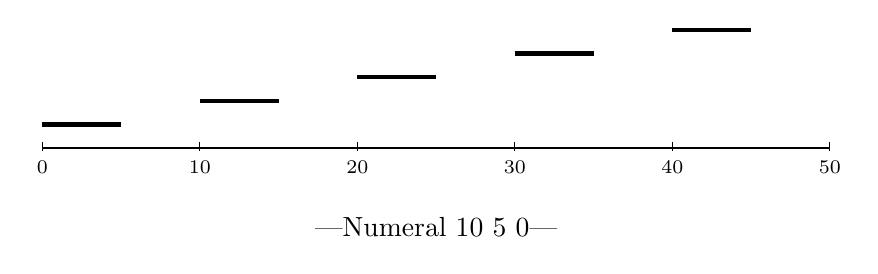
\begin{tikzpicture}
            % a straight line segment
            \draw (0, 0) -- (10, 0);
            % the ticks and their labels
            \foreach \x  in {0,...,5}
                \draw[xshift=\x*2 cm] (0pt,2pt) -- (0pt,-1pt) node[below,fill=white] {\scriptsize\the\numexpr\x*10\relax};
            \foreach \x  in {0,...,4}
                \draw[ultra thick, xshift=\x*2 cm, yshift=\x*0.3 cm] (0,0.3) -- (1,0.3);
            % labels
            \node at (5, -1) {{\lstinline|Numeral 10 5 0|}};
        \end{tikzpicture}
    \end{adjustbox}
\end{center}

Whilst systems such as {\lstinline|Numeral 10 15 0|} map more than one numeral
onto the same number. We can see immediately that their evaluations are not
\textit{injective} as those number lines ``overlap'' with each other.

\begin{center}
    \begin{adjustbox}{max width=\textwidth}
        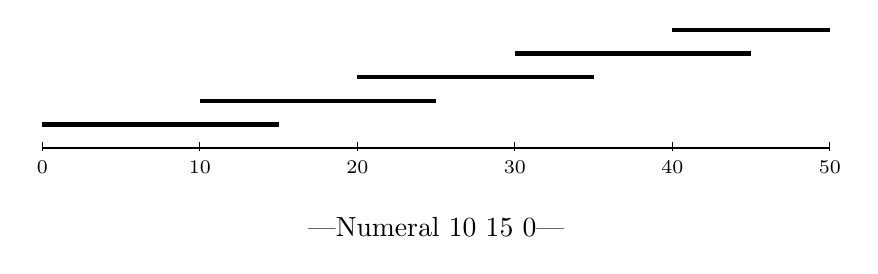
\begin{tikzpicture}
            % a straight line segment
            \draw (0, 0) -- (10, 0);
            % the ticks and their labels
            \foreach \x  in {0,...,5}
                \draw[xshift=\x*2 cm] (0pt,2pt) -- (0pt,-1pt) node[below,fill=white] {\scriptsize\the\numexpr\x*10\relax};
            \foreach \x  in {0,...,3}
                \draw[ultra thick, xshift=\x*2 cm, yshift=\x*0.3 cm] (0,0.3) -- (3,0.3);
            \draw[ultra thick, xshift=8 cm, yshift=1.2 cm] (0,0.3) -- (2,0.3);
            % labels
            \node at (5, -1) {{\lstinline|Numeral 10 15 0|}};
        \end{tikzpicture}
    \end{adjustbox}
\end{center}

As we can see, numerals do not align with numbers perfectly.
Finding ``the next number'' thus becomes a non-trivial problem.
Therefore, we define the next numeral as \textbf{the least numeral that is greater than itself}.

\subsection{Implementation}

Given a numeral, say {\lstinline|xs|}, to find the next numeral of {\lstinline|xs|},
it reasonable to expect that {\lstinline|xs|} must not be a maximum.
Otherwise, there would exist no such a numeral that is \textit{greater than itself}.

Again, the indices are classified by {\lstinline|numView|} into four categories.
The case of {\lstinline|NoDigits|} and {\lstinline|AllZeros|} are rather trivial.
We focus on the other two.

\begin{lstlisting}
next-number : ∀ {b d o}
    → (xs : Numeral b d o)
    → ¬ (Maximum xs)
    → Numeral b d o
next-number {b} {d} {o} xs ¬max with numView b d o
next-number xs ¬max | NullBase d o = ?
next-number xs ¬max | NoDigits b o = NoDigits-explode xs
next-number xs ¬max | AllZeros b   =
    contradiction (Maximum-AllZeros xs) ¬max
next-number xs ¬max | Proper b d o proper = ?
\end{lstlisting}

\subsection{Validating the Implementation}

To validate the correctness of the implementation of {\lstinline|next-number|},
i.e., to make sure that the function does return a numeral that is:

\begin{enumerate}
    \item greater than the given numeral
    \item the least of all such numerals
\end{enumerate}

We need to prove these two propositions:

\begin{lstlisting}
next-number-is-greater : ∀ {b d o}
    → (xs : Numeral b d o)
    → (¬max : ¬ (Maximum xs))
    → ⟦ next-number xs ¬max ⟧ > ⟦ xs ⟧
\end{lstlisting}

\begin{lstlisting}
next-number-is-immediate : ∀ {b d o}
    → (xs : Numeral b d o)
    → (ys : Numeral b d o)
    → (¬max : ¬ (Maximum xs))
    → ⟦ ys ⟧ > ⟦ xs ⟧
    → ⟦ ys ⟧ ≥ ⟦ next-number xs ¬max ⟧
\end{lstlisting}

We come up with the name ``immediate''
because ``the least numeral that is greater than itself'' is a bit too wordy.

\subsection{Outline}

We are going to finish programs and proofs of systems of {\lstinline|NullBase|}
and {\lstinline|Proper|} respectively.

\begin{itemize}
    \item {\lstinline|NullBase|}
        \begin{enumerate}
            \item {\lstinline|next-number-NullBase|}
            \item {\lstinline|next-number-is-greater-NullBase|}
            \item {\lstinline|next-number-is-immediate-NullBase|}
        \end{enumerate}
    \item {\lstinline|Proper|}
        \begin{itemize}
            \item {\lstinline|next-number-Proper|}
            \item {\lstinline|next-number-is-greater-Proper|}
            \item {\lstinline|next-number-is-immediate-Proper|}
        \end{itemize}
\end{itemize}

However, programs and proofs of systems of {\lstinline|Proper|} will be defined
\textit{simultaneously} with mutually recursive definitions.
The reason why we need properties like {\lstinline|next-number-is-greater-Proper|}
and {\lstinline|next-number-is-immediate-Proper|} in the first place is that
they are neccessary for implementing {\lstinline|next-number-Proper|}.

\subsection{The Next Numeral of NullBase}

To find the next numeral of systems of {\lstinline|NullBase|},
all we have to do is to manipulate the LSD.
Since only the value of the LSD has effect on the evaluation.
All numerals are mapped onto this single and continuous number line below.

\begin{center}
    \begin{tikzpicture}
        % a straight line segment
        \draw (0, 0) -- (10, 0);
        % the ticks and their labels
        \draw[xshift=0cm] (0pt,2pt) -- (0pt,-1pt) node[below,fill=white] {\the\numexpr0};
        % the thicker segment
        \draw[ultra thick] (1,0) -- (9,0);
        % the labels
        \node[fill=black,draw=black,circle,inner sep=2pt,label=above:{$o$}] at (1,0) {};
        \node[fill=black,draw=black,circle,inner sep=2pt,label=above:{$d+o$}] at (9,0) {};
        \node at (5, -0.5) {{\lstinline|ℕ|}};
    \end{tikzpicture}
\end{center}

Finding the next numeral is as simple as incrementing the LSD.
To make room for the increment, numerals that are mapped onto the rightmost
number of the line have to be excluded.

\begin{center}
    \begin{tikzpicture}
        % a straight line segment
        \draw (0, 0) -- (10, 0);
        % the ticks and their labels
        \draw[xshift=0cm] (0pt,2pt) -- (0pt,-1pt) node[below,fill=white] {\the\numexpr0};
        % the thicker segment
        \draw[ultra thick] (1,0) -- (8,0);
        % inner nodes
        \foreach \x in {2,...,7}
            \node[fill=black,draw=black,circle,inner sep=2pt](\x) at (\x,0) {};
        % labels
        \node[fill=black,draw=black,circle,inner sep=2pt,label=above:{$o$}](1) at (1,0) {};
        \node[fill=black,draw=black,circle,inner sep=2pt,label=above:{$d+o-1$}](8) at (8,0) {};
        \node[fill=white,draw=black,circle,inner sep=2pt,label=below:{$d+o$}](9) at (9,0) {};
        \node at (5, -1) {{\lstinline|ℕ|}};

        \foreach \x in {1,...,8} {
            \pgfmathsetmacro{\y}{\x + 1}
            \path[->,>=stealth']
                (\x) edge[bend right=60,transform canvas={xshift=-1pt, yshift=-3pt}] node [left] {} (\y);
        };
    \end{tikzpicture}
\end{center}

\subsubsection{{\lstinline|next-number-NullBase|}}

Numerals with the greatest LSD are first ruled out because they also happen
to be maxima. The rest of the numerals are then pattern matched to have their
LSDs replaced with an incremented one.

\begin{lstlisting}
next-number-NullBase : ∀ {d o}
    → (xs : Numeral 0 (suc d) o)
    → ¬ (Maximum xs)
    → Numeral 0 (suc d) o
next-number-NullBase xs       ¬max with Greatest? (lsd xs)
next-number-NullBase xs       ¬max | yes greatest =
    contradiction (Maximum-NullBase-Greatest xs greatest) ¬max
next-number-NullBase (x ∙)    ¬max | no ¬greatest =
    digit+1 x ¬greatest ∙
next-number-NullBase (x ∷ xs) ¬max | no ¬greatest =
    digit+1 x ¬greatest ∷ xs
\end{lstlisting}

\subsubsection{Lemma}

Instead of proving that {\lstinline|next-number-NullBase|} does compute a numeral
that is:
\begin{enumerate}
    \item greater than the given numeral
    \item the least of all such numerals
\end{enumerate}

We prove a stronger proposition, that {\lstinline|next-number-NullBase|} would
compute the \textit{successor} of the given number.

\begin{lstlisting}[basicstyle=\ttfamily\scriptsize]
next-number-NullBase-lemma : ∀ {d o}
    → (xs : Numeral 0 (suc d) o)
    → (¬max : ¬ (Maximum xs))
    → ⟦ next-number-NullBase xs ¬max ⟧ ≡ suc ⟦ xs ⟧
next-number-NullBase-lemma {d} {o} xs    ¬max with Greatest? (lsd xs)
next-number-NullBase-lemma {d} {o} xs    ¬max | yes greatest =
    contradiction (Maximum-NullBase-Greatest xs greatest) ¬max
next-number-NullBase-lemma {d} {o} (x ∙) ¬max | no ¬greatest =
    begin
        ⟦ digit+1 x ¬greatest ∙ ⟧
    ≡⟨ refl ⟩
        Digit-toℕ (digit+1 x ¬greatest) o
    ≡⟨ digit+1-toℕ x ¬greatest ⟩
        suc (Fin.toℕ x + o)
    ≡⟨ refl ⟩
        suc ⟦ x ∙ ⟧
    ∎
next-number-NullBase-lemma {d} {o} (x ∷ xs) ¬max | no ¬greatest =
    begin
        ⟦ digit+1 x ¬greatest ∷ xs ⟧
    ≡⟨ refl ⟩
        Digit-toℕ (digit+1 x ¬greatest) o + ⟦ xs ⟧ * zero
    ≡⟨ cong (λ w → w + ⟦ xs ⟧ * zero) (digit+1-toℕ x ¬greatest) ⟩
        suc (Fin.toℕ x + o + ⟦ xs ⟧ * zero)
    ≡⟨ refl ⟩
        suc ⟦ x ∷ xs ⟧
    ∎
\end{lstlisting}

\subsubsection{{\lstinline|next-number-is-greater-NullBase|}}

Recall that {\lstinline|x < y|} is essentially a synonym of {\lstinline|suc x ≤ y|}.
We nail this with the lemma we have just proven.

\begin{lstlisting}
next-number-is-greater-NullBase : ∀ {d o}
    → (xs : Numeral 0 (suc d) o)
    → (¬max : ¬ (Maximum xs))
    → ⟦ next-number-NullBase xs ¬max ⟧ > ⟦ xs ⟧
next-number-is-greater-NullBase xs ¬max =
    start
        suc ⟦ xs ⟧
    ≈⟨ sym (next-number-NullBase-lemma xs ¬max) ⟩
        ⟦ next-number-NullBase xs ¬max ⟧
    □
\end{lstlisting}

\subsubsection{{\lstinline|next-number-is-immediate-NullBase|}}

Here, the argument {\lstinline|ys|} stands for \textit{any} numeral of {\lstinline|Numeral 0 (suc d) o|}.

\begin{lstlisting}
next-number-is-immediate-NullBase : ∀ {d o}
    → (xs : Numeral 0 (suc d) o)
    → (ys : Numeral 0 (suc d) o)
    → (¬max : ¬ (Maximum xs))
    → ⟦ ys ⟧ > ⟦ xs ⟧
    → ⟦ ys ⟧ ≥ ⟦ next-number-NullBase xs ¬max ⟧
next-number-is-immediate-NullBase xs ys ¬max prop =
    start
        ⟦ next-number-NullBase xs ¬max ⟧
    ≈⟨ next-number-NullBase-lemma xs ¬max ⟩
        suc ⟦ xs ⟧
    ≤⟨ prop ⟩
        ⟦ ys ⟧
    □
\end{lstlisting}

\subsection{The Next Numeral of Proper}

Unlike in systems of {\lstinline|NullBase|} where every numeral gets mapped onto
a single and continuous number line.
Things are way more complicated in systems of {\lstinline|Proper|}.

% \subsubsection{Interior Numerals}


\begin{center}
    \begin{adjustbox}{max width=\textwidth}
        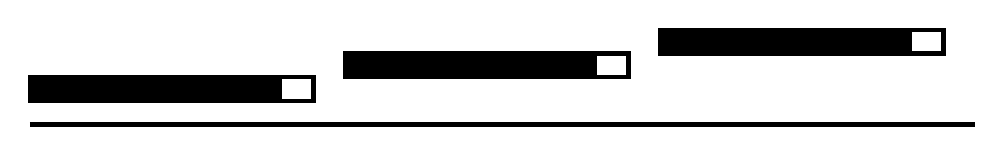
\begin{tikzpicture}
            \draw[ultra thick] (0, 0) -- (12, 0);
            %     \draw[xshift=\x*4 cm] (0pt,2pt) -- (0pt,-1pt) node[below,fill=white] {\scriptsize\the\numexpr\x*10\relax};

            % ticks
            % \foreach \i  in {0,...,30} {
            %     \draw[xshift=\i*0.4 cm] (0,0) -- (0,-0.2);
            % }
            % \foreach \i  in {0,...,3} {
            %     \draw[xshift=\i*4 cm, ultra thick] (0,0) -- (0,-0.3);
            % };

            \foreach \i  in {0,...,2} {
                \draw[xshift=\i*4 cm, yshift=\i*0.3 cm, ultra thick] (0, 0.3) rectangle (3.6, 0.6);
                \draw[xshift=\i*4 cm, yshift=\i*0.3 cm, fill=black] (0, 0.3) rectangle (3.2, 0.6);
            };
        \end{tikzpicture}
    \end{adjustbox}
\end{center}

% \subsubsection{Interior Numerals}

\begin{center}
    \begin{adjustbox}{max width=\textwidth}
        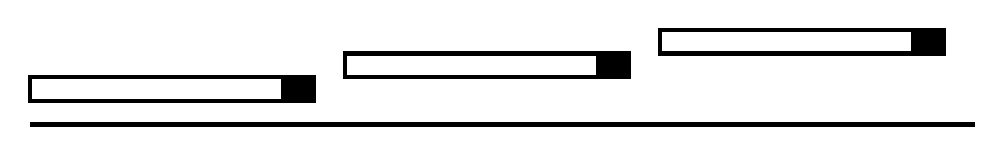
\begin{tikzpicture}
            \draw[ultra thick] (0, 0) -- (12, 0);
            \foreach \i  in {0,...,2} {
                \draw[xshift=\i*4 cm, yshift=\i*0.3 cm, ultra thick] (0, 0.3) rectangle (3.6, 0.6);
                \draw[xshift=\i*4 cm, yshift=\i*0.3 cm, fill=black] (3.2, 0.3) rectangle (3.6, 0.6);
            };
        \end{tikzpicture}
    \end{adjustbox}
\end{center}

\begin{center}
    \begin{adjustbox}{max width=\textwidth}
        \begin{tikzpicture}
            \draw[ultra thick] (0, 0) -- (12, 0);
            \path[clip] (0, -1) rectangle (12, 2);

            \foreach \i in {0,...,2} {
                \draw[xshift=\i*4cm, yshift=\i*0.3 cm, ultra thick] (0, 0.3) rectangle (4.4, 0.6);

                \foreach \j in {0,...,10} {
                    % \pgfmathsetmacro{\k}{\i * 11 + \j};
                    % \node (\k) at ({\k * 0.4 + 0.2}, {\i*0.3 + 0.2}) {.};
                    % \draw [->] (2) to [bend left] node[auto] {} (6);
                    % \path[->,>=stealth'] (1) edge[bend right] node [left] {} (12);
                    % \path [->] (12) to [bend left] node[auto] {} (16);

                    % \coordinate (\k) at ({\k}, 0.6);
                    % \path[->,>=stealth'] (1) edge[bend right=60] node [left] {} (20);
                    % \node[xshift=\i*4cm +\j*0.4cm, yshift=\i*0.3 cm] (\k) {\k};
                };
                \draw[xshift=\i*4 cm, yshift=\i*0.3 cm, fill=black] (4, 0.3) rectangle (4.4, 0.6);
            };

            \coordinate (A) at (4.2, 0.3);
            \coordinate (11) at (4.6, 0.3);
            \coordinate (1A) at (8.2, 0.6);
            \coordinate (21) at (8.6, 0.6);

            % \foreach \i in {0,...,11} {
            %     \coordinate (\i) at ({\i * 0.4 + 0.2}, 0.3);
            % }
            %
            % \foreach \i in {11,...,20} {
            %     \coordinate (\i) at ({\i * 0.4 + 0.2}, 0.6);
            % }
            %
            % \foreach \i in {21,...,29} {
            %     \coordinate (\i) at ({\i * 0.4 + 0.2}, 0.6);
            % }


            \path[->, thick] (A) edge[bend right=60] node {} (11);
            \path[->,>=stealth'] (1A) edge[bend right=60] node {} (21);
            % \path[->,>=stealth'] (10) edge[bend right] node {} (20);
            % \foreach \i  in {0,...,2} {
            %     \draw[xshift=\i*4 cm, yshift=\i*0.3 cm, ultra thick] (0, 0.3) rectangle (4.4, 0.6);
            %     % \draw[xshift=\i*4 cm, yshift=\i*0.3 cm, fill=black] (4, 0.3) rectangle (4.4, 0.6);
            %     % \pgfmathsetmacro{\next}{\i + 1};
            %     \path[->,>=stealth'] (1) edge[bend right=60] node [left] {} (2);
            % };


        % \foreach \x in {1,...,8} {
        %     \pgfmathsetmacro{\y}{\x + 1}
        %     \path[->,>=stealth']
        %         (\x) edge[bend right=60,transform canvas={xshift=-1pt, yshift=-3pt}] node [left] {} (\y);
        % };
        \end{tikzpicture}
    \end{adjustbox}
\end{center}


% \begin{center}
%     \begin{tikzpicture}
%         % a straight line segment
%         \draw (0, 0) -- (10, 0);
%         % the ticks and their labels
%         \draw[xshift=0cm] (0pt,2pt) -- (0pt,-1pt) node[below,fill=white] {\the\numexpr0};
%         % the thicker segment
%         \draw[ultra thick] (1,0) -- (9,0);
%         % the labels
%         \node[fill=black,draw=black,circle,inner sep=2pt,label=above:{$o$}] at (1,0) {};
%         \node[fill=black,draw=black,circle,inner sep=2pt,label=above:{$d+o$}] at (9,0) {};
%         \node at (5, -0.5) {{\lstinline|ℕ|}};
%     \end{tikzpicture}
% \end{center}



% There are three cases in {\lstinline|Proper|} we need to ha.

% Revisit the view function {\lstinline|numView|}.
% First, it pattern matches on {\lstinline|d|}, excluding systems with no digits;
% and then on {\lstinline|b|}, exluding systems with bases of $ 0 $.
% There is an order of pattern matching on the three indices.
%
\end{document}
